%!TEX root =../../course-notes.tex
% ^ leave for LaTeXTools build functionality

\begin{module}{A}{Algebraic properties of linear maps}

\begin{moduleStandards}
  \item \textbf{A1. Linear maps as matrices}
         I can write the matrix (with respect to the standard bases) corresponding to a linear transformation between Euclidean spaces.
  \item \textbf{A2. Linear map verification}
        I can determine if a map between vector spaces is linear or not.
  \item \textbf{A3. Injectivity and Surjectivity}
        I can determine if a given linear map is injective and/or surjective
  \item \textbf{A4. Kernel and Image}
        I can compute the kernel and image of a linear map, including finding bases.
\end{moduleStandards}


%!TEX root =../../course-notes.tex
% ^ leave for LaTeXTools build functionality

\begin{readinessAssuranceOutcomes}
\item Solve a system of linear equations (including finding a basis of the solution space if it is homogeneous) by interpreting as an augmented matrix and row reducing \standardList{E1, E2, E3, E4}.
\item State the definition of linear independence, and determine if a set of vectors is linearly dependent or independent \standardList{V5}.
\item State the definition of a spanning set, and determine if a set of vectors spans a vector space or subspace \standardList{V6, V7}.
\item State the definition of a basis, and determine if a set of vectors is a basis \standardList{V8, V9}.
\end{readinessAssuranceOutcomes}

\begin{readinessAssuranceResources}
\item TODO
\end{readinessAssuranceResources}




\begin{readinessAssuranceTest}

\item Which of the following is a solution to the system of linear equations
      \begin{align*}
      x+3y-z    &=   2 \\
      2x+8y+3z  &=  -1 \\
      -x-y+9z   &= -10
      \end{align*}

\begin{multicols}{4}
\begin{readinessAssuranceTestChoices}
\item $\begin{bmatrix} 1 \\ 1 \\ 0 \end{bmatrix}$
\item $\begin{bmatrix} 0 \\ 1 \\ -1 \end{bmatrix}$
\item $\begin{bmatrix} 1 \\ 0 \\ -1 \end{bmatrix}$
\item $\begin{bmatrix} 1 \\ -1 \\ 1 \end{bmatrix}$
\end{readinessAssuranceTestChoices}
\end{multicols}


\item Find a basis for the solution set of the following homogeneous system of
      linear equations
      \begin{align*}
      x+2y+-z-w    &= 0 \\
      -2x-4y+3z+5w &= 0
      \end{align*}

\begin{multicols}{4}
\begin{readinessAssuranceTestChoices}
\item $\left\{ \begin{bmatrix} 2 \\ 1 \\ 0 \\ 0 \end{bmatrix}, \begin{bmatrix} 2 \\ 0 \\ 3 \\ 1 \end{bmatrix} \right\}$
\item $\left\{ \begin{bmatrix} 2 \\ 2 \\ 0 \\ 0 \end{bmatrix}, \begin{bmatrix} 0 \\ 0 \\ 3 \\ 0 \end{bmatrix} \right\}$
\item $\left\{ \begin{bmatrix} 2 \\ 1 \\ 3 \\ 1 \end{bmatrix} \right\}$
\item None of these are a basis.
\end{readinessAssuranceTestChoices}
\end{multicols}


\item Determine which property applies to the set of vectors $$\left\{ \begin{bmatrix}  1 \\ 0 \\ 0 \end{bmatrix}, \begin{bmatrix} 0 \\ 1 \\ 0 \end{bmatrix} \right\} \subset \IR^3.$$

\begin{readinessAssuranceTestChoices}
\item It does not span and is linearly dependent
\item It does not span and is linearly independent
\item It spans but it is linearly dependent
\item It is a basis of $\IR^3$.
\end{readinessAssuranceTestChoices}


\item Determine which property applies to the set of vectors $$\left\{ \begin{bmatrix}  1 \\ 0 \\ 0 \end{bmatrix}, \begin{bmatrix} 2 \\ 1 \\ 0 \end{bmatrix} , \begin{bmatrix} 1 \\ 1 \\ 3 \end{bmatrix} \right\}\subset \IR^3.$$

\begin{readinessAssuranceTestChoices}
\item It does not span and is linearly dependent
\item It does not span and is linearly independent
\item It spans but it is linearly dependent
\item It is a basis of $\IR^3$.
\end{readinessAssuranceTestChoices}


\item Determine which property applies to the set of vectors $$\left\{ \begin{bmatrix}  1 \\ 0 \\ 0 \end{bmatrix}, \begin{bmatrix} -2 \\ 0 \\ -2 \end{bmatrix} , \begin{bmatrix} 1 \\ 1 \\ 0 \end{bmatrix} , \begin{bmatrix} 3 \\ 3 \\ -3 \end{bmatrix}\right\}\subset \IR^3.$$

\begin{readinessAssuranceTestChoices}
\item It does not span and is linearly dependent
\item It does not span and is linearly independent
\item It spans but it is linearly dependent
\item It is a basis of $\IR^3$.
\end{readinessAssuranceTestChoices}


\item Determine which property applies to the set of vectors $$\left\{ \begin{bmatrix}  2 \\ 2 \\ -1 \end{bmatrix}, \begin{bmatrix} -3 \\ 1 \\ -2 \end{bmatrix} , \begin{bmatrix} 1 \\ 5 \\ -4 \end{bmatrix}\right\}\subset \IR^3.$$

\begin{readinessAssuranceTestChoices}
\item It does not span and is linearly dependent
\item It does not span and is linearly independent
\item It spans but it is linearly dependent
\item It is a basis of $\IR^3$.
\end{readinessAssuranceTestChoices}


\item Find a basis for the subspace of $\IR^4$ spanned by the vectors ...


\item Suppose you know that every vector in $\IR^5$ can be written as a linear combination of the vectors $\{\vec{v}_1, \ldots, \vec{v}_n\}$.  What can you conclude about $n$?

\begin{readinessAssuranceTestChoices}
\item $n \leq 5$
\item $n=5$
\item $n \geq 5$
\item $n$ could be any positive integer
\end{readinessAssuranceTestChoices}

\item Suppose you know that every vector in $\IR^5$ can be written uniquely as a linear combination of the vectors $\{\vec{v}_1, \ldots, \vec{v}_n\}$.  What can you conclude about $n$?

\begin{readinessAssuranceTestChoices}
\item $n \leq 5$
\item $n=5$
\item $n \geq 5$
\item $n$ could be any positive integer
\end{readinessAssuranceTestChoices}

\item Suppose you know that every vector in $\IR^5$ can be written uniquely as a linear combination of the vectors $\{\vec{v}_1, \ldots, \vec{v}_n\}$.  What can you conclude about the set $\{\vec{v}_1, \ldots, \vec{v}_n\}$?

\begin{readinessAssuranceTestChoices}
\item It does not span and is linearly dependent
\item It does not span and is linearly independent
\item It spans but it is linearly dependent
\item It is a basis of $\IR^3$.
\end{readinessAssuranceTestChoices}

\end{readinessAssuranceTest}

%!TEX root =../../course-notes.tex
% ^ leave for LaTeXTools build functionality

\begin{applicationActivities}{1}{17}

\begin{definition}
A \term{linear transformation} is a map between vector spaces that preserves the vector space operations.  More precisely, if $V$ and $W$ are vector spaces, a map $T:V\rightarrow W$ is called a linear transformation if
\begin{enumerate}
\item $T(\vec{v}+\vec{w}) = T(\vec{v})+T(\vec{w})$ for any $\vec{v},\vec{w} \in V$
\item $T(c\vec{v}) = cT(\vec{v})$ for any $c \in \IR$, $\vec{v} \in V$.
\end{enumerate}
In other words, a map is linear if one can do vector space operations before applying the map or after, and obtain the same answer.
\end{definition}

\begin{definition}
Given a linear transformation \(T:V\to W\),
$V$ is called the \term{domain} of $T$ and
$W$ is called the \term{co-domain} of $T$.

\begin{center}
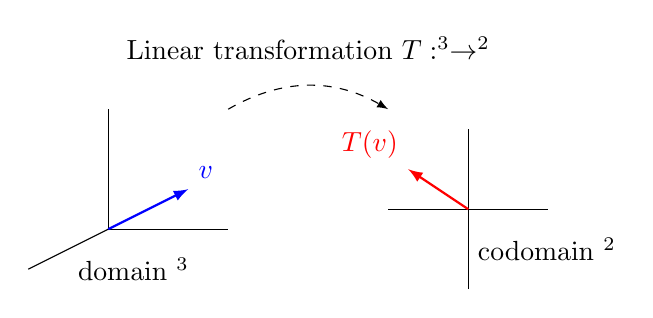
\begin{tikzpicture}[x=0.2in,y=0.2in]
  \begin{scope}[shift={(0,0)}]
    \draw (0,0) -- (3,0);
    \draw (0,0) -- (0,3);
    \draw (0,0) -- (-2,-1);
    \draw[thick,-latex,blue] (0,0) -- (2,1)
          node[anchor=south west] {\(\vect v\)};
    \node[anchor=west] at (-1,-1) {domain \(\IR^3\)};
  \end{scope}
  \draw[dashed,-latex] (3,3) to [bend left=30] (7,3);
  \node[anchor=south] at (5,4) {Linear transformation \(T:\IR^3\to\IR^2\)};
  \begin{scope}[shift={(9,0.5)}]
    \draw (-2,0) -- (2,0);
    \draw (0,-2) -- (0,2);
    \draw[thick,-latex,red] (0,0) -- (-1.5,1)
          node[anchor=south east] {\(T(\vect v)\)};
    \node[anchor=west] at (0,-1) {codomain \(\IR^2\)};
  \end{scope}
\end{tikzpicture}
\end{center}
\end{definition}

\begin{example}
Let $T : \IR^3 \rightarrow \IR^2$ be given by $$T\left(\begin{bmatrix} x \\ y \\ z \end{bmatrix} \right) = \begin{bmatrix} x-z \\ y \end{bmatrix}$$

\pause To show that \(T\) is linear, we must verify...
\[
  T\left(
    \begin{bmatrix} x_1 \\ y_1 \\ z_1 \end{bmatrix} +
    \begin{bmatrix}x_2 \\ y_2  \\ z_2 \end{bmatrix}
  \right)
=
  T\left(
    \begin{bmatrix} x_1+x_2 \\ y_1+y_2 \\ z_1+z_2 \end{bmatrix}
  \right) =
  \begin{bmatrix} (x_1+x_2)-(z_1+z_2) \\ (y_1+y_2) \end{bmatrix}
\]
\[
  T\left(
    \begin{bmatrix} x_1 \\ y_1 \\ z_1 \end{bmatrix}
  \right) + T\left(
    \begin{bmatrix} x_2 \\ y_2 \\ z_2 \end{bmatrix}
  \right)
=
  \begin{bmatrix} x_1-z_1 \\ y_1 \end{bmatrix} +
  \begin{bmatrix} x_2-z_2 \\ y_2 \end{bmatrix}=
  \begin{bmatrix} (x_1+x_2)-(z_1+z_2) \\ (y_1+y_2) \end{bmatrix}
\]
\pause
And also...
\[
  T\left(c\begin{bmatrix} x \\ y \\ z \end{bmatrix} \right)
=
  T\left(\begin{bmatrix} cx \\ cy \\ cz \end{bmatrix} \right)
=
  \begin{bmatrix} cx-cz \\ cy \end{bmatrix}
\text{ and }
  cT\left(\begin{bmatrix} x \\ y \\ z \end{bmatrix} \right)
=
  c\begin{bmatrix} x-z \\ y \end{bmatrix}
=
  \begin{bmatrix} cx-cz \\ cy \end{bmatrix}
\]

Therefore $T$ is a linear transformation.
\end{example}


\begin{activity}{15}
Determine if each of the following maps are linear transformations
\begin{subactivity}
$T_1: \IR^2 \rightarrow \IR$ given by $T_1 \left(\begin{bmatrix} x \\ y \end{bmatrix} \right) = \sqrt{x^2+y^2}$.
\end{subactivity}
\begin{subactivity}
$T_2: \IR^3 \rightarrow \IR^3 $ given by $T_2\left(\begin{bmatrix} x \\ y \\ z \end{bmatrix} \right)  = \begin{bmatrix} -x \\ -y \\ -z \end{bmatrix}$
\end{subactivity}
\begin{subactivity}
$T_3: \P^d \rightarrow \P^{d-1}$ given by $T_3(f(x)) = f^\prime(x)$.
\end{subactivity}
\begin{subactivity}
$T_4: \P \rightarrow \P$ given by $T_4(f(x)) = f(x)+x^2$
\end{subactivity}
\end{activity}

\begin{activity}{5}
Suppose $T: \IR^3 \rightarrow \IR^2$ is a linear transformation, and you know $T\left(\begin{bmatrix} 1 \\ 0 \\ 0 \end{bmatrix} \right) = \begin{bmatrix} 2 \\ 1 \end{bmatrix} $ and $T\left(\begin{bmatrix} 0 \\ 0 \\ 1 \end{bmatrix} \right) = \begin{bmatrix} -3 \\ 2 \end{bmatrix} $.  Compute $T\left(\begin{bmatrix} 3 \\ 0 \\ 0 \end{bmatrix}\right)$.
\begin{multicols}{2}
\begin{enumerate}[(a)]
\item $\begin{bmatrix} 6 \\ 2\end{bmatrix}$
\item $\begin{bmatrix} -9 \\ 6 \end{bmatrix}$
\item $\begin{bmatrix} -4 \\ -2 \end{bmatrix}$
\item $\begin{bmatrix} 6 \\ 4 \end{bmatrix}$
\end{enumerate}
\end{multicols}
\end{activity}

\begin{activity}{3}
Suppose $T: \IR^3 \rightarrow \IR^2$ is a linear transformation, and you know $T\left(\begin{bmatrix} 1 \\ 0 \\ 0 \end{bmatrix} \right) = \begin{bmatrix} 2 \\ 1 \end{bmatrix} $ and $T\left(\begin{bmatrix} 0 \\ 0 \\ 1 \end{bmatrix} \right) = \begin{bmatrix} -3 \\ 2 \end{bmatrix} $.  Compute $T\left(\begin{bmatrix} 0 \\ 0 \\ -2 \end{bmatrix}\right)$.
\begin{multicols}{2}
\begin{enumerate}[(a)]
\item $\begin{bmatrix} 6 \\ 2\end{bmatrix}$
\item $\begin{bmatrix} -9 \\ 6 \end{bmatrix}$
\item $\begin{bmatrix} -4 \\ -2 \end{bmatrix}$
\item $\begin{bmatrix} 6 \\ 4 \end{bmatrix}$
\end{enumerate}
\end{multicols}
\end{activity}

\begin{activity}{5}
Suppose $T: \IR^3 \rightarrow \IR^2$ is a linear transformation, and you know $T\left(\begin{bmatrix} 1 \\ 0 \\ 0 \end{bmatrix} \right) = \begin{bmatrix} 2 \\ 1 \end{bmatrix} $ and $T\left(\begin{bmatrix} 0 \\ 0 \\ 1 \end{bmatrix} \right) = \begin{bmatrix} -3 \\ 2 \end{bmatrix} $.  Compute $T\left(\begin{bmatrix} 1 \\ 0 \\ 1 \end{bmatrix}\right)$.
\begin{multicols}{2}
\begin{enumerate}[(a)]
\item $\begin{bmatrix} 2 \\ 1\end{bmatrix}$
\item $\begin{bmatrix} 3 \\ -1 \end{bmatrix}$
\item $\begin{bmatrix} -1 \\ 3 \end{bmatrix}$
\item $\begin{bmatrix} 5 \\ -8 \end{bmatrix}$
\end{enumerate}
\end{multicols}
\end{activity}

\begin{activity}{2}
Suppose $T: \IR^3 \rightarrow \IR^2$ is a linear transformation, and you know $T\left(\begin{bmatrix} 1 \\ 0 \\ 0 \end{bmatrix} \right) = \begin{bmatrix} 2 \\ 1 \end{bmatrix} $ and $T\left(\begin{bmatrix} 0 \\ 0 \\ 1 \end{bmatrix} \right) = \begin{bmatrix} -3 \\ 2 \end{bmatrix} $.  Compute $T\left(\begin{bmatrix} -2 \\ 0 \\ -3 \end{bmatrix}\right)$.
\begin{multicols}{2}
\begin{enumerate}[(a)]
\item $\begin{bmatrix} 2 \\ 1\end{bmatrix}$
\item $\begin{bmatrix} 3 \\ -1 \end{bmatrix}$
\item $\begin{bmatrix} -1 \\ 3 \end{bmatrix}$
\item $\begin{bmatrix} 5 \\ -8 \end{bmatrix}$
\end{enumerate}
\end{multicols}
\end{activity}

\begin{activity}{5}
Suppose $T: \IR^4 \rightarrow \IR^3$ is a linear transformation.
How many facts of the form $T(\vec{v}_i)=\vec{w}_i$ do you need to know in order to be able to compute $T(\vec{v})$ for \textit{any} $\vec{v} \in \IR^4$?
\begin{enumerate}[(a)]
\item $2$
\item $3$
\item $4$
\item $5$
\item You need infinitely many
\end{enumerate}
(In this situation, we say that the vectors \(\{\vect v_1,\dots,\vect v_n\}\)
\term{determine} \(T\).)
\end{activity}

\begin{fact}
Consider any basis \(\{\vect b_1,\dots,\vect b_n\}\) for $V$.  Since every vector can be written \textit{uniquely} as a linear combination of basis vectors, every linear transformation $T:V \rightarrow W$ is determined by those basis vectors.

\[
  T(\vect v)=T(x_1\vect b_1+\dots x_n\vect b_n)=
  x_1T(\vect b_1)+\dots+x_nT(\vect b_n)
\]
\end{fact}

\begin{definition}
The \term{standard basis} of $\IR^n$ is the (ordered) basis $\{\vec{e}_1, \vec{e}_2, \ldots, \vec{e}_n\}$ where
\begin{align*}
\vec{e}_1 &= \begin{bmatrix} 1 \\ 0 \\ 0 \\\vdots \\ 0 \\ 0 \end{bmatrix}  &
\vec{e}_2 &= \begin{bmatrix} 0 \\ 1 \\ 0 \\\vdots \\ 0 \\ 0 \end{bmatrix}  & \cdots  & &
\vec{e}_n &= \begin{bmatrix} 0 \\ 0 \\ 0 \\\vdots \\ 0 \\ 1 \end{bmatrix}
\end{align*}

Since linear transformation \(T:\IR^n\to\IR^m\) is determined by
the values of each \(T(\vec e_i)\), it's convenient to store this
information in the \(m\times n\) matrix
\([T(\vec e_1) \,\cdots\, T(\vect e_n)]\).
\end{definition}


\begin{example}
Let $T: \IR^3 \rightarrow \IR^2$ be the linear transformation determined by
the following values for \(T\) applied to the standard basis of \(\IR^3\).
\begin{align*}
T\left(\begin{bmatrix} 1 \\ 0 \\ 0 \end{bmatrix} \right) &= \begin{bmatrix} 3 \\ 2\end{bmatrix} &
T\left(\begin{bmatrix} 0 \\ 1 \\ 0 \end{bmatrix} \right) &= \begin{bmatrix} -1 \\ 4\end{bmatrix} &
T\left(\begin{bmatrix} 0 \\ 0 \\ 1 \end{bmatrix} \right) &= \begin{bmatrix} 5 \\ 0\end{bmatrix}
\end{align*}

Then the matrix corresponding to $T$ with respect to the standard bases is $$\begin{bmatrix}3 & -1 & 5 \\ 2 & 4 & 0 \end{bmatrix}.$$
\end{example}

\begin{activity}{5}
  Let $T: \IR^3 \rightarrow \IR^2$ be the linear transformation given by
$$T\left(\begin{bmatrix} x\\ y \\ z \end{bmatrix} \right) = \begin{bmatrix} x+3z \\ 2x-y-4z \end{bmatrix}$$
Write the matrix corresponding to this linear transformation with respect to the standard basis.
\end{activity}

\begin{activity}{5}
  Let $T: \IR^3 \rightarrow \IR^2$ be the linear transformation given by the matrix (with respect to the standard bases) $$\begin{bmatrix} 3  & -2 & -1  \\ 4 & 5 & 2 \end{bmatrix}.$$

Compute $T\left(\begin{bmatrix} x\\ y \\ z \end{bmatrix} \right) $.
\end{activity}

% \begin{fact}
%   $T: \IR^n \rightarrow \IR^m$ is given by the matrix
%   \([\vect v_1 \,\cdots\, \vect v_n]\) exactly when
%   \(T\left(
%     \begin{bmatrix}
%       x_1 \\ \vdots \\ x_n
%     \end{bmatrix}
%   \right)
%     =
%   x_1\vect v_1 + \dots + x_n\vect v_n\).
% \end{fact}

\begin{activity}{10}
Let $D: \P^3 \rightarrow \P^2$ be the derivative map \(D(f(x))=f'(x)\).
(Earlier we showed this is a linear transformation.)
\begin{subactivity}
Write down an equivalent linear transformation $T: \IR^4 \rightarrow \IR^3$
by converting \(\{1,x,x^2,x^3\}\) and \(\{D(1),D(x),D(x^2),D(x^3)\}\) into
appropriate vectors in \(\IR^4\) and \(\IR^3\).
\end{subactivity}
\begin{subactivity}
Write the matrix corresponding to $T$ with respect to the standard bases.
\end{subactivity}
\end{activity}

\end{applicationActivities}

%!TEX root =../../course-notes.tex
% ^ leave for LaTeXTools build functionality

\begin{applicationActivities}{2}{19}

\begin{definition}
Let $T: V \rightarrow W$ be a linear transformation.
\begin{itemize}
\item $T$ is called \term{injective} or \term{one-to-one} if $T$ does not map two distinct values to the same place.  More precisely, $T$ is injective if $T(\vec{v}) \neq T(\vec{w})$ whenever $\vec{v} \neq \vec{w}$.
\item $T$ is called \term{surjective} or \term{onto} if every element of $W$ is mapped to by an element of $V$.  More precisely, for every $\vec{w} \in W$, there is some $v \in V$ with $T(\vec{v})=\vec{w}$.
\end{itemize}
\end{definition}

\begin{activity}{0}
Let $T: \IR^3 \rightarrow \IR^2$ be given by the matrix $\begin{bmatrix} 1 & 0 \\ 0 & 1 \\ 0 & 0 \end{bmatrix}$.  Determine if $T$ is injective, surjective, both, or neither.
\end{activity}

\begin{activity}{0}
Let $T: \IR^2 \rightarrow \IR^3$ be given by the matrix $\begin{bmatrix} 1 & 0 &0  \\ 0 & 1 & 0 \end{bmatrix}$.  Determine if $T$ is injective, surjective, both, or neither.
\end{activity}

\begin{definition}
We also have two important sets called the \term{kernel} of $T$ and the \term{image} of $T$.
\begin{align*}
\ker T &= \left\{ \vec{v} \in V\ \big|\ T(\vec{v})=0\right\} \\
\Im T &= \left\{ \vec{w} \in W\ \big|\ \text{there is some }v\in V \text{ with } T(\vec{v})=\vec{w}\right\}
\end{align*}
\end{definition}

\begin{activity}{0}
Let $T: \IR^3 \rightarrow \IR^2$ be given by the matrix $\begin{bmatrix} 1 & 0 \\ 0 & 1 \\ 0 & 0 \end{bmatrix}$ (for the standard basis).  Find the kernel and image of $T$.
\end{activity}

\begin{activity}{0}
Let $T: \IR^2 \rightarrow \IR^3$ be given by the matrix $\begin{bmatrix} 1 & 0 &0  \\ 0 & 1 & 0 \end{bmatrix}$ (for the standard basis).  Find the kernel and image of $T$.
\end{activity}

\begin{activity}{0}
  \begin{subactivity}
    Describe surjective linear transformations in terms of the image.
  \end{subactivity}
  \begin{subactivity}
    Describe injective linear transformations in terms of the kernel.
  \end{subactivity}
\end{activity}

\begin{activity}{0}
Let $T: \IR^3 \rightarrow \IR^2$ be the linear transformation given by the matrix $A=\begin{bmatrix} 3 & 4 & -1 \\ 1 & 2 & 1 \end{bmatrix}$ (for the standard basis).
\begin{enumerate}[1)]
\item Write a system of equations whose solution set is the kernel.
\item Compute $\RREF(A)$ and solve the system of equations.
\item Compute the kernel of $T$
\item Find a basis for the kernel of $T$
\end{enumerate}
\end{activity}

\begin{activity}{0}
Let $S: \IR^3 \rightarrow \IR^2$ be the linear transformation given by the matrix $B=\begin{bmatrix} 3 & 4 & 1 \\ 1 & 2 & 4 \\ 5 & 8 & 9 \end{bmatrix}$ (for the standard basis).
\begin{enumerate}[1)]
\item Write a system of equations whose solution set is the kernel.
\item Compute $\RREF(A)$ and solve the system of equations.
\item Compute the kernel of $T$
\item Find a basis for the kernel of $T$
\end{enumerate}
\end{activity}

\begin{activity}{0}
Let $T: \IR^3 \rightarrow \IR^3$ be the linear transformation given by the matrix $A=\begin{bmatrix} 3 & 4 & -1 \\ 1 & 2 & 1 \end{bmatrix}$ (for the standard basis).
\begin{enumerate}[1)]
\item Find a set of vectors that span the image of $T$
\item Find a basis for the image of $T$.
\end{enumerate}
\end{activity}

\begin{activity}{0}
Let $S: \IR^3 \rightarrow \IR^3$ be the linear transformation given by the matrix $B=\begin{bmatrix} 3 & 4 & 1 \\ 1 & 2 & 4 \\ 5 & 8 & 9  \end{bmatrix}$ (for the standard basis).
\begin{enumerate}[1)]
\item Find a set of vectors that span the image of $T$
\item Find a basis for the image of $T$.
\end{enumerate}
\end{activity}

\end{applicationActivities}

%!TEX root =../../course-notes.tex
% ^ leave for LaTeXTools build functionality

\begin{applicationActivities}{Day 3}

\begin{activity}{0}
Let $T: \IR^n \rightarrow \IR^m$ be a linear map with matrix $A \in M_{m,n}$ (for the standard basis).  You have cards containing a number of statements about $T$ and $A$.  Sort them into groups of equivalent statements, and post them on your board.

\begin{TBLnote}Card sort activity for 10-15 minutes: cards contain the following
\begin{enumerate}[(a)]
\item $T$ is injective
\item $T$ is not injective
\item $T$ is surjective
\item $T$ is not surjective
\item The system of linear equations given by the augmented matrix $\begin{bmatrix}[c|c]A & \vec{b} \end{bmatrix}$ has a solution for all $\vec{b} \in \IR^m$
\item The system of linear equations given by the augmented matrix $\begin{bmatrix}[c|c]A & \vec{b} \end{bmatrix}$ has a unique solution for all $\vec{b} \in \IR^m$
\item The system of linear equations given by the augmented matrix $\begin{bmatrix}[c|c] A & \vec{0} \end{bmatrix}$ has a non-trivial solution.
\item The columns of $A$ span $\IR^m$
\item The columns of $A$ are linearly independent
\item The columns of $A$ are a basis of $\IR^m$
\item Every column of $\RREF(A)$ is a pivot column
\item $\RREF(A)$ has a non-pivot column
\item $\RREF(A)$ has $n$ pivot columns
\end{enumerate}
\end{TBLnote}
\end{activity}

\begin{activity}{0}
\begin{TBLnote}Gallery walk \end{TBLnote}
Cycle around the room counter-clockwise.  If they have two things grouped together that you know are not equivalent, write a reason or counter-example on a sticky note.
\end{activity}

\begin{activity}{0}
Come up with as many statements as you can, and add them to the appropriate group.
\end{activity}

\end{applicationActivities}


\end{module}
